\clearpage
\section{Use Case Diagram Design}

\subsection{Actors}

The Decentralized Smart Power Grid system involves three primary actors:

\begin{itemize}
    \item Consumer
    \item Grid Administrator
    \item Smart Meter (ESP32)
\end{itemize}

The consumer monitors electricity usage, manages prepaid balance, and receives notifications. The administrator supervises system operations, monitors alerts, and manages consumers. The smart meter continuously sends energy consumption data to the backend.
\subsection{Use Case Diagram}

The use case diagram illustrates the interactions between external actors and the major functionalities provided by the Decentralized Smart Power Grid System.

\begin{figure}[H]
    \centering
    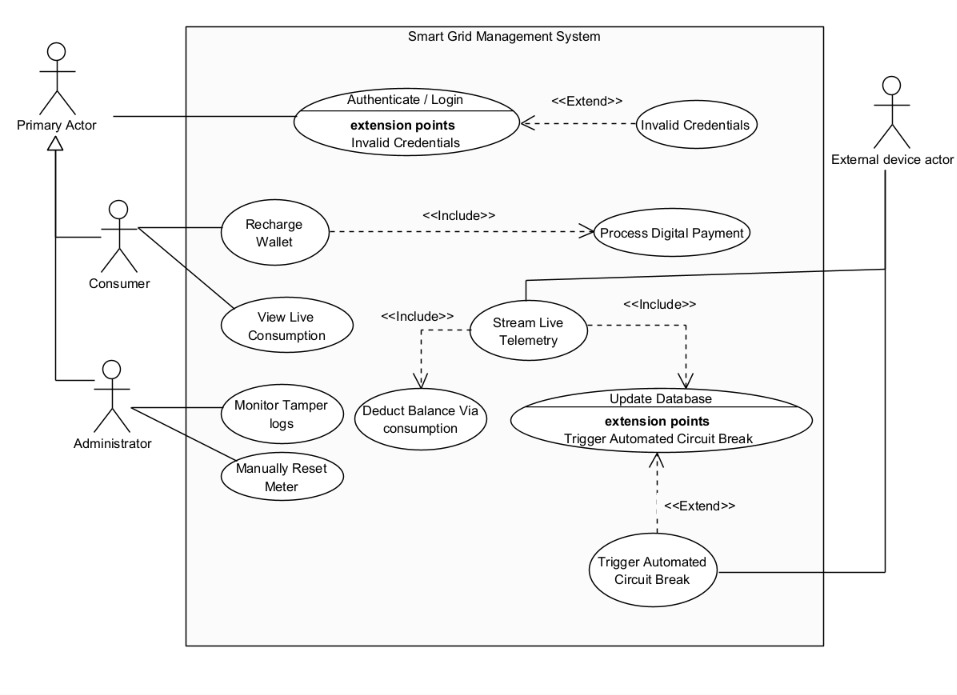
\includegraphics[width=0.95\textwidth]{graphics/usecase.jpeg}
    \caption{Use Case Diagram of the Decentralized Smart Power Grid System}
\end{figure}

\subsection{Use Case Description}

The diagram shows how consumers interact with the system to monitor energy consumption, recharge prepaid balances, and receive notifications, while administrators monitor grid status and manage consumers. The smart meter supplies real-time telemetry to support automated billing and monitoring.